\chapter{Evaluation}
% Ergebinsse der Untersuchung
Im nachfolgenden Kapitel werden neben der Untersuchung auf Erfüllung der in Kapitel \ref{sec:anforderungsanalyse} erarbeiteten Anforderungen auch die Vor- und Nachteile, die in dieser Arbeit aufgekommen sind aufgezeigt.

\section{Interpretation der Ergebnisse der Untersuchung}
\label{sec:untersuchung}
In Kapitel \ref{chap:untersuchung} wurde beschrieben, wie die Anwendung auf Erfüllung der Anforderungen untersucht wird. Nachfolgend werden die Ergebnisse der Untersuchung aufgezeigt.

\subsection{Beurteilung der technischen Realisierung}
Das Durchlaufen der einzelnen Testfälle hat ergeben, dass nicht alle der funktionalen Anforderungen im Prototypen bereits vollständig realisiert wurden.

Die ersten zwei Anforderungen werden vollumfänglich erfüllt. Die Anzahl aktiver Mitarbeiter lässt sich variieren und es werden auch nur die entsprechend relevantem \textit{\glspl{Timesheet}} in das neue Verzeichnis kopiert. auch wird an dem Dateinamen nichts verändert. Dazu wurde eine Methode geschrieben, die die Dateinamen der kopierten Dateien entsprechend der Vorgaben setzt. Auch der Monat ist bereits anpassbar, jedoch in der aktuellen Anwendungsversion noch als Variable im Code und nicht in der Konfigurationsdatei selbst. Das anzupassen sollte jedoch kein großer Aufwand sein.

Auch der Test mit einem besonders großen \gls{Timesheet} war erfolgreich, genauso wie bei manueller Überprüfung keine Verlusten innerhalb der Dateien festgestellt werden konnten.

Das von \gls{Spring Boot} bereitgestellte Logging deckt nicht die gewünschten Anforderungen ab. An dieser Stelle muss der Code manuell angepasst werden und weiteres Logging in den zutreffenden Funktionen implementiert werden. Genauso wird die Anwendung in ihrer aktuellen Version bei einem Fehler sofort beendet und ist noch nicht in der Lage das Kopieren fehlerhafter \textit{\glspl{Timesheet}} zu überspringen. \pagebreak

Eine Anpassung der Rootverzeichnisses dagegen ist jedoch ohne Probleme möglich, solange die in dem Verzeichnis befindliche Ordnerstruktur den Vorgaben entspricht.

Damit ist ein großer Teil der funktionalen Anforderungen bereits in diesem Prototypen erfüllt, das korrekte Logging und Fehlerhandling sind jedoch für eine zukünftige Anwendungsversion unumgänglich.

\subsection{Untersuchung der nicht-funktionalen Anforderungen}
\textbf{Skalierbarkeit:}

Der vorliegende Prototyp ist durch die von \ac{ECS} bereitgestellten Funktionalitäten horizontal Skalierbar. Es können zu jedem Zeitpunkt weitere Container gestartet werden, um die Anwendung zu skalieren. Genauso werden diese bei Inaktivität wieder entfernt. \\

\textbf{Fehlertoleranz:}

Die Fehlertoleranz der Anwendung wird in \ac{ECS} ebenfalls gewährleistet. Stürzt ein Container ab oder wird unerwartet beendet, wird automatisch ein neuer Container gestartet um den Workload abzufangen. \\

\textbf{Schnelle Bereitstellung:}

Durch den Einsatz von \textit{CodePipeline} kann jede Anwendungsaktualisierung nahezu in Echtzeit bereitgestellt werden. Wird der Anwendungscode aktualisiert (es reicht zum Testen das hinzufügen eines Kommentars), startet automatisch ein neues Deployment und die Anwendung wird aktualisiert. \\

\textbf{Mehrbenutzerfähigkeit:}

Die Mehrbenutzerfähigkeit der Anwendung ist bereits in \gls{Spring Boot} gegeben, da in \gls{Spring Boot}-Anwendungen standardmäßig mehrere Personen auf eine Anwendungsinstanz zugreifen können. Hierfür stellt \gls{Spring Boot} bzw. der darunter laufende Anwendungsserver einen Pool von \textit{Threads} bereit. Wird ein \textit{Request} durch einen Nutzer ausgelöst, wird dieser durch einen \textit{Thread} verarbeitet. Greift ein weiterer Nutzer auf die Anwendung zu, wird ein weiterer \textit{Thread} beansprucht. Wurde eine Anfrage abgeschlossen, wird der \textit{Thread} wieder Teil des Pools. \pagebreak

\textbf{Sicherheit:}

Die Sicherheitsanforderungen an die Anwendung werden trotz aktuell verwendeter Testdatensätze bereits umgesetzt oder sind nachträglich leicht umsetzbar. Die Cloud Infrastruktur ist in einem \ac{VPC} mit privatem Subnet implementiert, welches in sich geschlossen ist. Das API-Gateway ermöglicht zudem zusätzliche Authentifizierungsmöglichkeiten, die jedoch für den Test des Prototypen deaktiviert wurden. Darüber hinaus können auch in \gls{Spring Boot} Module zur Prüfung von Nutzerberechtigungen mithilfe von \textit{Spring Security} und zum Beispiel JWT Token eingesetzt werden. Damit sind die in der Public Cloud möglichen Sicherheitsstandards umgesetzt. Bei der Sensibilität der realen Anwendungsdaten ist jedoch zu untersuchen, ob diese als ausreichend erachtet werden.

\subsection{Beurteilung der finanziellen Aspekte}
Um die oberflächliche finanzielle Betrachtung zu beurteilen, folgt zuerst die Berechnung der geschätzten anfallenden Kosten, bevor diese gegeneinander aufgewogen werden um einschätzen zu können, ob oder wann sich die Cloud Migration der untersuchten Anwendung lohnt.

\textbf{Ursprüngliche Anwendung:}

\begin{align}
    Installationszeit = \frac{4 \times 0,02h \times 20}{Jahr} = \frac{1,6h}{Jahr}
\end{align}

Die Installationszeit ergibt sich aus ungefähr 4 Updates, die pro Jahr heruntergeladen werden müssen. Dabei wird der Zeitaufwand auf eine Minute pro Update geschätzt. Bei ungefähr 20 Anwendern ergeben sich 48 Personenstunden pro Jahr für die Installation der Anwendung.

\begin{align}
    Installationskosten = \frac{1,6h}{Jahr} \times \frac{1000\mbox{\euro}}{8h} =\frac{200\mbox{\euro}}{Jahr}
\end{align}

Für einen durchschnittlichen Nutzer der Anwendung werden ungefähr 1000Euro pro Tag kalkuliert und durch 8 Arbeitsstunden pro Tag geteilt. \pagebreak

% \begin{align}
%     Updatezeit: \frac{4}{Jahr} \times \left(1min \times 20\right) = \frac{80min}{Jahr}
% \end{align}

% Zur Kalkulation des benötigten Zeitaufwand wird mit 4 Updates/Jahr, die ausgerollt werden. Als benötigte Zeit wird hier eine Minute für das aktualisieren des \gls{Repository} geschätzt. Bei ungefähr 20 Anwendern macht das 80 Minuten/Jahr.

% \begin{align}
%     Ausführungszeit: \frac{720}{Jahr} \times \left(2min \times 20\right)  = \frac{28.800min}{Jahr}
% \end{align}

% Um die Ausführungszeit für die Anwendung schätzen zu können, wird davon ausgegangen, dass diese 12x/Jahr, immer am Monatsende ausgeführt wird. Bei ungefähr 60 Ausführungen, von denen jede einzelne ungefähr zwei Minuten braucht und ebenfalls von 20 Personen durchgeführt wird, ergibt das 28.800 Minuten/Jahr (480h/Jahr).

% \begin{align}
%     Entwicklungszeit: \frac{4800min}{Jahr}
% \end{align}

% Die Entwicklungszeit ist schwer vorherzusagen, es ist jedoch zu schätzen, dass der Entwickler ungefähr an 30 Tagen im Jahr zwischen 3 und 4 Stunden in die Weiterentwicklung der Anwendung investiert, was eienen Schätzwert von 80h/Jahr ergibt.

% \begin{align}
%     Zeitaufwand = Updatezeit + Ausführungszeit + Entwicklungszeit = \\
%     \frac{80min}{Jahr} + \frac{28.800min}{Jahr} + \frac{4.800min}{Jahr} = \frac{33.680min}{Jahr}
% \end{align}

% Der Zeitaufwand summiert sich also zu 560 Personenstunden/Jahr. Davon ausgegangen, dass ein durchschnittlicher Consultant ca. 5.500€/Monat verdient, kosten 560 Personenstunden knapp 15.000€/Jahr. \\

\textbf{Migrierte Anwendung:}

Für die migrierte Anwendung entfallen der Aufwand und die damit verbundenen Kosten zur Installation und Aktualisierung dieser. Dieser Prozess ist durch die Bereitstellung in der Cloud und das automatisierte Deployment der Anwendung durch eine Pipeline realisiert. Stattdessen fallen für den Betrieb der Cloud Infrastruktur jedoch Kosten von Jährlich ca. 900€ pro Jahr an. Diese ergeben sich aus ca. 75\$ pro Monat laut \ac{AWS}-Preisrechner. Durch den aktuellen Kurs des Euro (1€ = 1\$ [Stand: 29.08.2022]) ist der Wert eins zu eins übertragbar.

\begin{figure}[H]
    \centering
    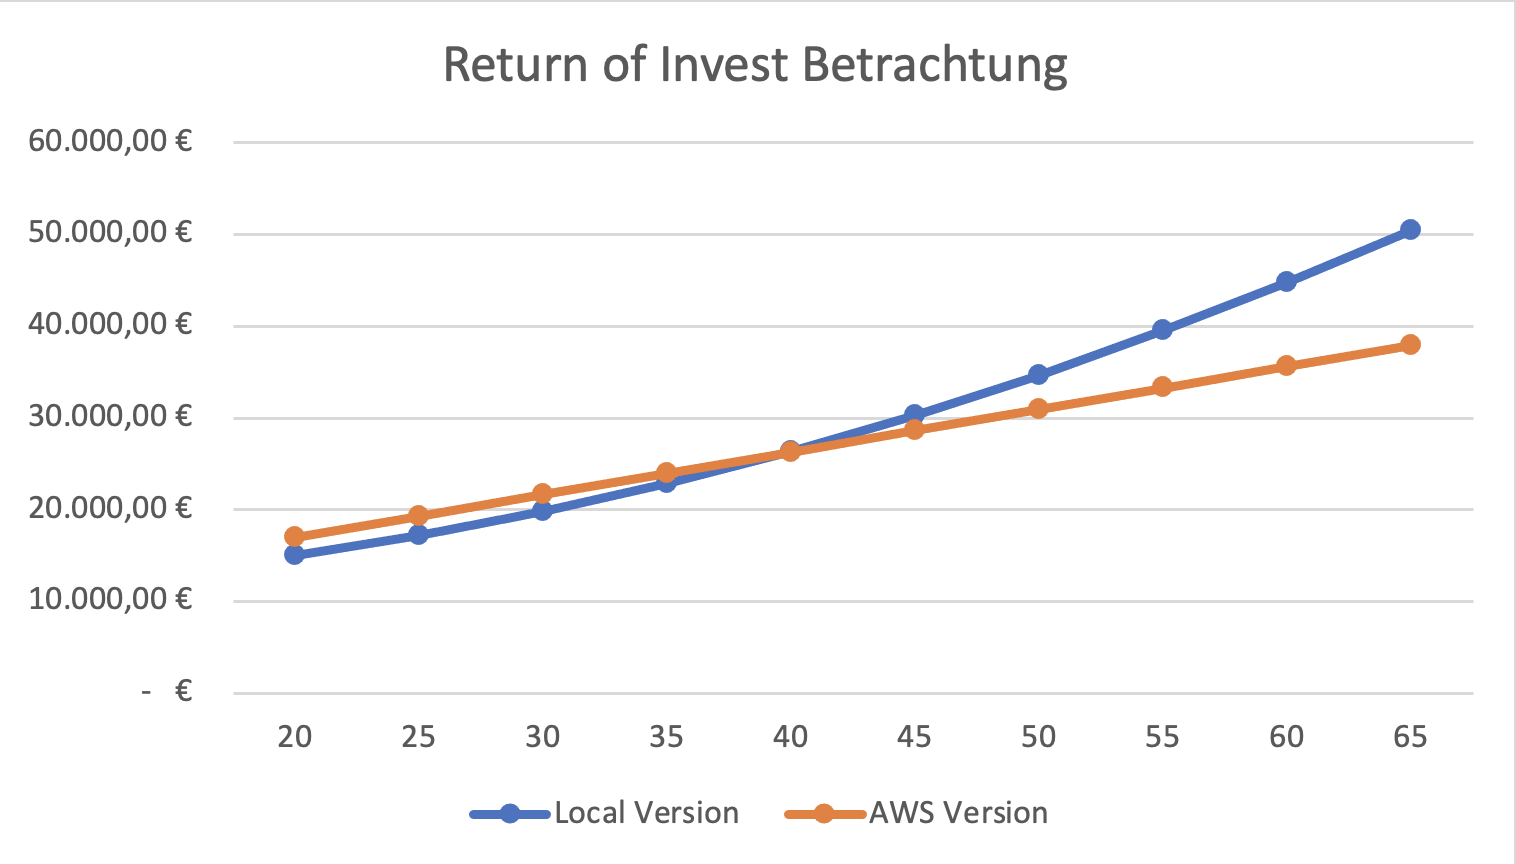
\includegraphics[width=\textwidth]{roi.png}
    \caption{Return of Invest Betrachtung: Break-Even bei ca. 40 Anwendern}
    \label{fig:roi}
\end{figure}

% \begin{align}
%     Updatezeit: \frac{0min}{Jahr}
% \end{align}

% Die Updatezeit für die migrierte Anwendung fällt durch die Bereitstellung in der Cloud auf Null.

% \begin{align}
%     Ausführungszeit: \frac{720}{Jahr} \times \left(2min \times 20\right)  = \frac{28.800min}{Jahr}
% \end{align}

% Bei der Ausführungszeit wird davon ausgegangen, dass diese sich trotz einiger Änderungen an der Anwendung nicht stark ändern wird.

% \begin{align}
%     Entwicklungszeit: \frac{4800min}{Jahr} + 3.000min = \frac{7.800min}{Jahr}
% \end{align}

% Die Grundlegende Entwicklungszeit wird sich ebenfalls nicht verändern, jedoch ergänzt, durch die erforderliche Zeit zur Migration der Anwendung. Dabei sind ca. 10 Stunden für das erste Modul verwendet worden und es wird von mindestens der doppelten Entwicklungszeit für die weiteren Module ausgegangen, da diese wesentlich komplexere Logik enthalten.

% \begin{align}
%     Zeitaufwand = Updatezeit + Ausführungszeit + Entwicklungszeit = \\
%     \frac{0min}{Jahr} + \frac{28.800min}{Jahr} + \frac{7.800min}{Jahr} = \frac{36.600min}{Jahr}
% \end{align}

% Für das erste Jahr mit der migrierten Anwendung werden ca. 610 Personenstunden erwartet, was Kosten von ungefähr 16.100€/Jahr ergibt. Zusätzlich dazu sind außerdem noch die Betriebskosten für die Cloud Infrastruktur einzukalkulieren, die laut \ac{AWS}-Preisrechner bei ca. 75\$/Monat und somit 900\$/Jahr erwartet ergeben. Bei dem aktuellen Kurs des Euro (1€ = 1\$ [Stand: 29.08.2022]) ergeben das insgesamt 17.000€/Jahr.

% Durch diese Kalkulation ergibt sich, dass die Kosten für die Cloud Migration der untersuchte Anwendung im ersten Jahr definitiv höher sind, als die Anwendung einfach weiter zu betreiben. Für die  weitere Entwicklung der Kosten, kann mit einer Break-Even Analyse untersucht werden, ab welcher Benutzerzahl sich eine Migration der Anwendung in die Cloud rentieren würde. Dazu wird von einem Jährlichen Zuwachs von ungefähr 20 weiteren Nutzern ausgegangen, in der Annahme, dass die Anwendung zukünftig auch in weiteren Projekten eingesetzt wird.
\pagebreak

\section{Vor- und Nachteile der Cloud Migration}
Wie einleitend in dieser Arbeit aufgezeigt, nutzen immer mehr Unternehmen das Cloud Computing in den verschiedensten Unternehmensbereichen. Nachfolgend soll bewertet werden, in welcher Form sich Vor- und Nachteile aus der in dieser Arbeit untersuchten Migration ergeben haben und wie diese sich auf das Gesamtbild der Cloud Migration übertragen lassen.

\subsection{Vorteile}
Aus der beispielhaften Migration des \textit{Collect Service} in die Cloud ergeben sich folgende Vorteile für die Anwendung:

In der Cloud bereitgestellt ist der Service fortan rund um die Uhr verfügbar und unabhängig von der ausführenden Maschine. Es ist nicht mehr notwendig die Anwendung auf einem lokalen Rechner zu installieren (oder einen Rechner zu verwenden, wo diese bereits installiert ist) und jeder Benutzer kann diese nun, unabhängig vom lokalen Betriebssystem, über eine \ac{API} erreichen. Statt des \ac{API}-Endpoints könnte der Prozess außerdem zum Beispiel über einen Batch-Job oder einen Trigger automatisiert werden.

Updates der Anwendung werden automatisiert über die \ac{CI/CD}-Pipeline deployed und müssen nicht mehr manuell durchgeführt werden. Damit entfällt der Aufwand, vor jeder Nutzung die Aktualität der Anwendung zu überprüfen für alle Anwender und diese erhalten automatisch die neueste Version der Anwendung. So können zum Beispiel Bugfixes schneller und einfacher ausgerollt werden. 

Darüber hinaus bietet sich bei lokalen Anwendungen, wie der in dieser Arbeit untersuchten, eine Benutzeroberfläche nicht unbedingt an. Durch die Umwandlung dieser zu einer Web-Anwendung und Bereitstellung in der Cloud ergeben sich hier neue Möglichkeiten, wie zum Beispiel eine Ausführung der Anwendung über ein beliebiges mobiles Endgerät (z. B. Smartphone) oder einer grafischen Oberfläche um auch für weniger technische Nutzer eine einfache Bedienbarkeit zu bieten. \pagebreak

\subsection{Nachteile}
Neben den positiven Aspekten die bei der Migration in die Cloud aufgekommen sind, haben sich auch einige Nachteile ergeben:

Das Rebuilding einer Anwendung bringt, bevor die Anwendung fertig entwickelt ist, zuerst einen großen Entwicklungsaufwand mit sich. Ein Entwickler muss die Funktionen der Anwendung verstehen und reproduzieren ohne, dass Funktionen aus der ursprünglichen Anwendung verloren gehen. Dieser Aufwand war mit dem in dieser Arbeit untersuchten \textit{Collect Service} zwar noch nicht allzu groß, jedoch ist bereits bei diesem Aufgefallen, dass noch nicht alle logischen Bausteine entsprechend reproduziert wurden. Die übrigen Services übertreffen den \textit{Collect Service} in ihrer Komplexität um ein vielfaches, da diese unter anderem Makros aus Excel verarbeiten können und viele Daten aufeinander abstimmen müssen.

Darüber hinaus ist die Gewährleistung der Sicherheitsanforderungen und der Schutz der Daten zwar grundsätzlich innerhalb der Cloud-Umgebung möglich und auch innerhalb der Anwendungen zu implementieren, jedoch nicht ohne weitere Aufwände, was in sicherheitskritischen Fällen zu kostenintensiven Positionen führen kann. 

Im Falle der hier untersuchten Anwendung sollte außerdem hinterfragt werden, ob die im vorangehenden Kapitel aufgezeigten Vorteile die Betriebskosten für den Cloud Provider aufwiegen. Den teaminternen Informationen nach ist das für diese Anwendung nicht der Fall, solange die Benutzerzahl nicht deutlich ansteigt. Individuelle Aufwände und Betriebskosten werden hier in einer Höhe eingeschätzt, die sich nicht rechtfertigen lassen. Desweiteren muss bei der Migration in eine andere Programmiersprache erneut eine vollständige Qualitätssicherung der Anwendung durchgeführt werden, da der Anspruch and die Richtigkeit der erzeugten Dokumente extrem hoch ist.
\pagebreak